\documentclass[11pt,a4j]{jarticle}

\newcommand{\setcounters}[1] {
  \setcounter{equation}{#1}
  \setcounter{figure}{#1}
  \setcounter{table}{#1}
}

\newcommand{\unit}[1] {
  \hspace{1mm}\mathrm{[#1]}
}

\newcommand{\degc} {
  \hspace{1mm}\mathrm{[}{}^\circ\mathrm{C]}
}

\newcommand{\refig}[1]{図\ref{fig::#1}}
\newcommand{\refeq}[1]{式(\ref{eq::#1})}
\newcommand{\reftab}[1]{表\ref{tab::#1}}

\newcommand{\fig}[5] {
  \begin{figure}[#1]
    \begin{center}
      \includegraphics[width=#2\hsize]{#3}
    \end{center}
    \caption{#4}
    \label{fig::#5}
  \end{figure}
}

\makeatletter
\def\eq{\@ifstar\@eq\@@eq}
\def\@eq#1{\begin{equation*}#1\end{equation*}}
\def\@@eq#1#2{\begin{equation}#2\label{eq::#1}\end{equation}}
\makeatother

\newcommand{\diff}[2] {
  \frac{\mathrm{d}#1}{\mathrm{d}#2}
}

\newcommand{\pdiff}[2] {
  \frac{\partial #1}{\partial #2}
}


\newcommand{\ddt}[2][1] {
  \ifnum #1 < 2
    \frac{\mathrm{d}#2}{\mathrm{d}t}
  \else
    \frac{\mathrm{d}^#1#2}{\mathrm{d}t^#1}
  \fi
}

\newcommand{\e}[1] {
  \mathrm{e}^{#1}
}

\newcommand{\lparen}{(}
\catcode `( = \active
\newcommand{(}{\ifmmode\left\lparen\else\lparen\fi}

\newcommand{\rparen}{)}
\catcode `) = \active
\newcommand{)}{\ifmmode\right\rparen\else\rparen\fi}

\newcommand{\bmat}[1] {
  \begin{bmatrix} #1 \end{bmatrix}
}

% -- Package ---------------------------------------------------
\usepackage[dvipdfmx]{graphicx}
\usepackage{amsmath, amssymb}
\usepackage{bm}
\usepackage{fancyhdr}
\usepackage{here}
\usepackage{listings}
\usepackage{multirow}


% -- Margin Config ---------------------------------------------
\setlength{\textheight}{\paperheight}
\setlength{\topmargin}{4.6truemm} % 30mm(=1.0in+4.6mm)
\addtolength{\topmargin}{-\headheight}
\addtolength{\topmargin}{-\headsep}
\addtolength{\textheight}{-60truemm}

\setlength{\textwidth}{\paperwidth}
\setlength{\oddsidemargin}{-0.4truemm} % 25mm(=1.0in-0.4mm)
\setlength{\evensidemargin}{-0.4truemm}
\addtolength{\textwidth}{-50truemm}


% -- Renewcommand ----------------------------------------------
\renewcommand{\theequation}{\arabic{section}.\arabic{equation}}
\renewcommand{\thefigure}{\arabic{figure}}
\renewcommand{\thetable}{\thesection.\arabic{table}}
\renewcommand{\lstlistingname}{ソースコード}
\renewcommand{\headrulewidth}{0mm} % fancy
\renewcommand{\labelenumi}{(\arabic{enumi})}


% -- Config for fancy package ----------------------------------
\pagestyle{fancy}
\rhead{\thepage}
\lhead{}
\cfoot{}


% -- Config for package listings -------------------------------
\lstset{
  basicstyle={\ttfamily \small},
  breaklines=true,
  frame=trBL,
  numbers=left,
  numberstyle={\ttfamily \small},
}




\begin{document}
\begin{titlepage}

  \vspace*{25mm}

  \begin{center}
    {\huge 知能制御PBL\\}
    \vspace{10mm}
    {\Huge 第2回RCR中間報告\\}
    \vspace{20mm}
    {\Large 2018年6月6日}

    \vspace{15mm}

    {\LARGE 西田研究室\\}

    \vspace{15mm}

    {\Large
   13104042 烏谷崇大    \\
   14104055 佐々木秀将\\
   15104021 長田駿二郎\\
   15104026 川崎雄太朗\\
   15104050 坂元勇太    \\
   15104081 徳野将士    \\
   15104113 前田修一    \\
   15104117 右田明花    \\
   15104134 山福佳        \\
   17104311 横田篤紀    \\
}

  \end{center}

\end{titlepage}


\newpage
	\tableofcontents

\newpage

\section{目的}
	学部3年までに学習した制御理論や電気回路・情報工学の知識を使って,競技場内を自律的に走行するロボットの製作を行う.
	研究室で一丸となってプロジェクトを進行し,共同で課題を達成することの難しさや楽しさを学び,エンジニアとして仕事を進めるための素養を身に付ける.

\section{RCR (Robot Car Race) 2018}

\subsection{競技概要}
	ウレタンパネルを用いてレイアウトされる周回コースにおいて,格子模様のコントロールライン手前から走行開始してコントロールラインを3回通過後に停止するまでの時間を競うロボットカー(以下,ロボカーと称する)を製作する.

\subsection{コース}
一辺$50\unit{cm}$の正方形及び扇形の黒色ウレタンパネルと白黒格子模様のコントロールライン付ウレタンパネルを組み合わせ,コースを構成する.
なお,競技会当日までコースは公表されない.また,コースフェンスの高さが低いため,コースフェンスのコース側に高さ$10\unit{cm}$の壁を設置する.

\subsection{競技ルール}
	\begin{enumerate}
      \item コントロールライン手前からの走行開始からコントロールラインを3回通過後に停止するまでの時間を競う.
      \item 各チームあたり10分以内に最大3回走行し,最短時間の走行を評価する.
      \item コース2周以上走行すること.
      \item 競技会当日のコース試走は認めない.
      \item ロボカーがコース周囲の壁に接触した場合は失格とする.
      \item コース及び壁に物を設置したり,手を加えてはいけない.
      \item コース内に足を踏み入れないこと.

    \end{enumerate}

\newpage
\section{機体}
\refig{first}に配布されたロボカー本体の写真をしめす.\refig{fisrt}より本体の前方には前輪を駆動させ機体を旋回させるためのサーボモータを設置している.そして,本体の後方には後輪を駆動させ機体を動かすためのDCモータを設置し,その上にロータリエンコーダを設置した.

次に,\refig{second}に本体の上に設置するパーツの写真を,\refig{third}にその上に設置するパーツの写真示す.\refig{second}より中央にはDCモータを制御するためのモータドライバ,後方には各部品に電力を供給するためのバッテリ,前方にはRaspberry Pi3 model Bに電力を供給するためのモバイルバッテリを設置した.そして,前方と左右にコースの壁の距離を計測するためのPSDセンサを設置した.\refig{third}より,一番上にはRaspberry Pi3 model BとDC-DCコンバータを含めた電気回路を設置している.

そして,現在,配線が\refig{second},\refig{third}よりロボカー本体に他の部品を設置するためにユニバーサルプレートを採用した.その理由は最初に,加工しやすいからである.ユニバーサルプレートは素材がプラスチックで出来ているので切断しやすいという特徴がある.次に,様々な部品の取り外しや設置がやりやすいからである.ユニバーサルプレートには無数の穴が開いているので簡単にボルトとナットに部品を設置できる.また,プラスチックは電気を通しにくいので電気回路の絶縁にもなるからである.

最後に,\refig{forth}にロボカーの背面の写真を示す.\refig{forth}より,現在はまだ設置してないがロボカーの背面にゴールラインを読み取るためのフォトリフレクタを設置する予定である.

\begin{figure}[htb]
\centering
\includegraphics[width=0.5\hsize]{picture/eps/one.eps}
\caption{ロボカー本体}
\label{fig::first}
\end{figure}

\begin{figure}[htb]
\centering
\includegraphics[width=0.5\hsize]{picture/eps/two.eps}
\caption{ロボカー1段目}
\label{fig::second}
\end{figure}

\begin{figure}[htb]
\centering
\includegraphics[width=0.5\hsize]{picture/eps/three.eps}
\caption{ロボカー2段目}
\label{fig::third}
\end{figure}

\begin{figure}[htb]
\centering
\includegraphics[width=0.5\hsize]{picture/eps/four.eps}
\caption{ロボカー背面}
\label{fig::forth}
\end{figure}

\begin{figure}[h]
\centering
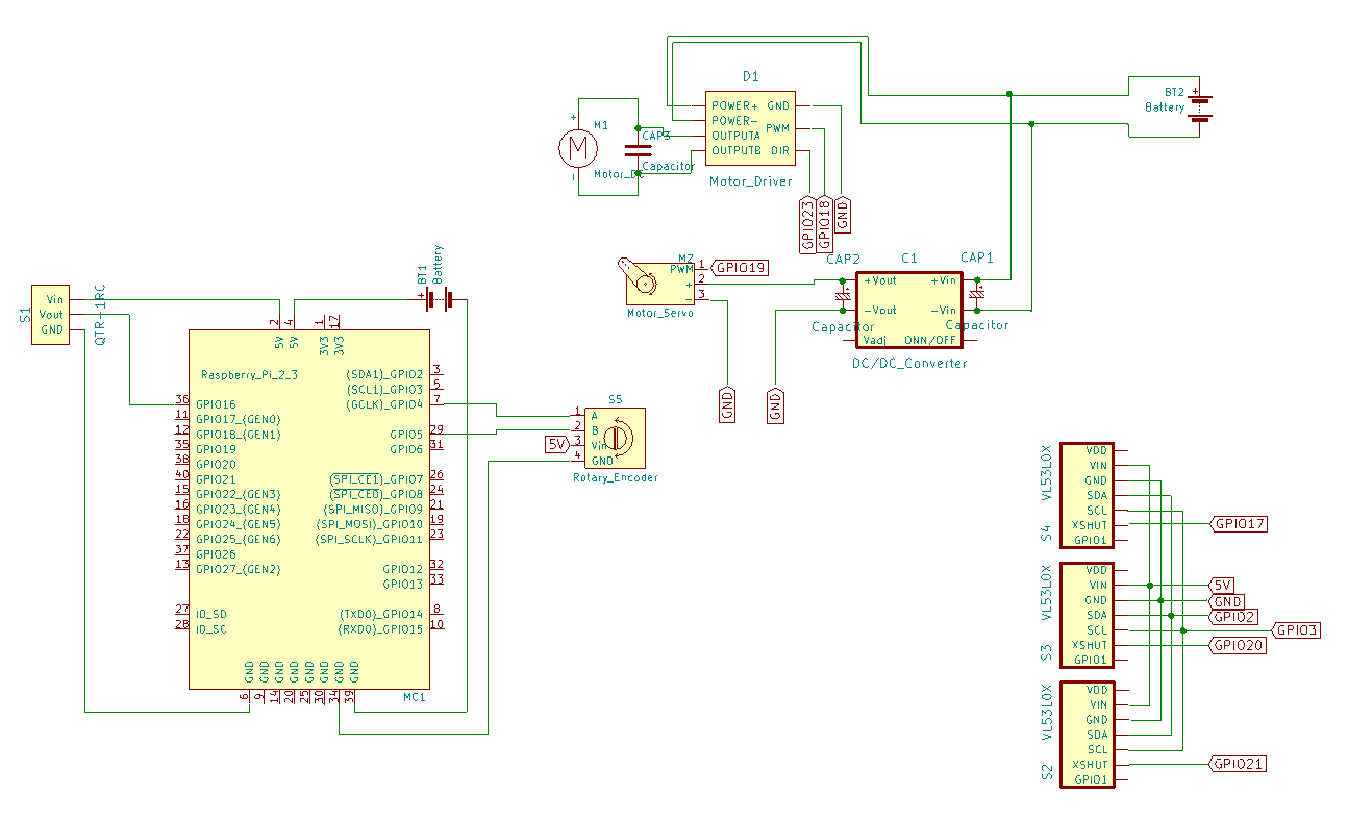
\includegraphics[scale=0.6]{picture/eps/ele_circuit_fig1.eps}
\caption{回路図}
\label{fig::overall_electric_circuit}
\end{figure}
\section{回路設計}
今回設計した回路を\refig{overall_electric_circuit},回路制作に使用した主要な部品の一覧を\reftab{circuit_parts}にそれぞれ示す.さらに各電子部品の仕様や構成について以下に示す.

\subsection{電源回路}
以下に示す仕様のようにRaspberryPi3 Model Bとサーボモータ,DCモータドライバではそれれぞれ定格電圧が異なるため同一の電源を用いることができない.そこで$7.2\unit{V}$バッテリと$5\unit{V}$バッテリの2つを用いている.
$7.2\unit{V}$バッテリはまず分流を行い,一方をDC-DCコンバータを用いて$7.2\unit{V}$から$5\unit{V}$に降圧してサーボモータに供給し,もう片方をDCモータドライバに供給している.$5\unit{V}$バッテリはRaspberryPi3 Model Bに電源を供給している.
\begin{description}
    \item[モータドライバ\textless MD10CR3\textgreater \cite{motordriver}]\mbox{}\\
    \vspace{-5mm}
        \begin{itemize}
            \item モータ電源電圧: DC $5\unit{V}-25\unit{V}$
            \item 最偉大電流  : $13\unit{A}$
            \item ロジック入力電圧: $3.3\unit{V}-5\unit{V}$
        \end{itemize}
    \item[サーボモータ\textless GWS03T/2BBMG\textgreater]\mbox{}\\
    \vspace{-5mm}
         \begin{itemize}
            \item 駆動電圧: DC $4.8\unit{V}-6\unit{V}$
        \end{itemize}
     \item[RaspberryPi3 ModelB\cite{rpi}]\mbox{}\\
     \vspace{-5mm}
         \begin{itemize}
            \item 電源: $5\unit{V}$,$2.5\unit{A}$
        \end{itemize}

\end{description}


\begin{table}
    \caption{電気回路用部品}
    \label{tab::circuit_parts}
    \begin{center}
    \footnotesize
   \begin{tabular}{ | l | l | c || l |}\hline
タイプ               &部品名                                         &数&用途   \\ \hline\hline
マイコン             &Raspberry Pi3 Model B                            &1&制御用           \\ \hline
DCモータ             &RP380-ST                                  &1&後輪モータ駆動用   \\    \hline
モータドライバ          &MD10C R3                                        &1&後輪モータ制御用   \\ \hline
距離センサ            &VL53L0X Time-of-Flight                           &3&距離計測用   \\ \hline
フォトリフレクタ         &QTR-1RC フォトリフレクタ・モジュール              &3&ゴールライン計測用   \\ \hline
DC-DCコンバータ          &BTD05-05S200D                                     &1&降圧用   \\ \hline
コンデンサ                &セラミックコンデンサ$1000\unit{pF}50\unit{V}$ &1&後輪モータのノイズ除去用   \\ \cline{2-4}
                          &OSコンデンサ $10\unit{V}47\unit{\mu F}$                          &2&DC-DCコンバータのノイズ除去用    \\ \hline
ロータリーエンコーダ   &RE30E-500-213-1                                   &1&ロボカーの速度計測用   \\ \hline
バッテリ             &Powers Max 4000 Ni-MH $7.2\unit{V}$                        &1&DCモータ,サーボモータ用の電源\\ \cline{2-4}
                          &$4000\unit{mAh}$ 6CELL ニッケル水素バッテリ                &1&Raspberry Pi3 ModelB用の電源    \\ \hline
サーボモータ           &GWS03T/2BBMG                                &1&ステアリング用   \\    \hline
 
	   \end{tabular} 
	\end{center}
\end{table}


\newpage

\begin{figure}[h!]
\centering
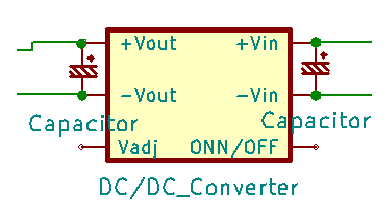
\includegraphics[scale=0.8]{picture/eps/ele_cap.eps}
\caption{DC-DCコンバータの回路図}
\label{fig::ele_cap}
\end{figure}

\subsection{DC-DCコンバータ}
本回路上で降圧を行うためにDC-DCコンバータを用いた.以下にその仕様を示す.DC-DCコンバータは内部でディジタルスイッチングを行っているため,ノイズが多い\cite{dcdc}.本回路ではこのようなノイズ成分を除去するために電解コンデンサ(OSコンデンサ$10\unit{V}47\unit{\mu F}$)を用いた\refig{ele_cap}の回路を作成した\cite{dcdcconverter}.
\begin{description}
    \item[DC-DCコンバータ\textless BTD05-05S200D\textgreater \cite{dcdcconverter}]\mbox{}\\
    \vspace{-5mm}
        \begin{itemize}
            \item 入力電圧: DC $4.5\unit{V}-9\unit{V}$
            \item 出力電圧: $0\unit{mA}-2000\unit{mA}$
            \item 出力電流: $3.3\unit{V}-5\unit{V}$
            \item 効率: 84 \%
        \end{itemize}
\end{description}



\newpage
\section{ROS (Robot Operating System)}
\subsection{ROSとは}
ROS(Robot Operating System)とはOpen Source Robotics Foundationによって管理されているソフトウェア開発者のロボット・アプリケーション作成を支援するフレームワークである.
具体的には,ハードウェア抽象化,デバイスドライバ,ライブラリ,視覚化ツール,メッセージ通信,パッケージ管理などが提供されている.つまりROSは汎用コンピュータ向けのOSではなく,汎用コンピュータ向けOS上で動作するメタOSとして捉えることができる\cite{kurazume}.

\refig{ros_topic}に示すようにROSではプロセス(実行プログラム)はノードという単位で扱い,ノード間の通信はトピックと呼ばれる``Publisher/Subscriber''モデルで実現される\cite{ogura}.

これにより,プログラミング言語や通信相手さえ意識することなく簡単にプロセス間通信を実現できる.
これは各ノード間のインタフェース,すなわちトピックの名前と型さえ決定すればノードごとに独立して開発を行うことができるという利点でもある.\\

以上の利点を考慮し,本研究室ではROSがインストール可能なマイコンボードであるRaspberryPi3 Model B上にROSをインストールして開発を進めていくこととした.

\begin{figure}[htb]
  \centering
    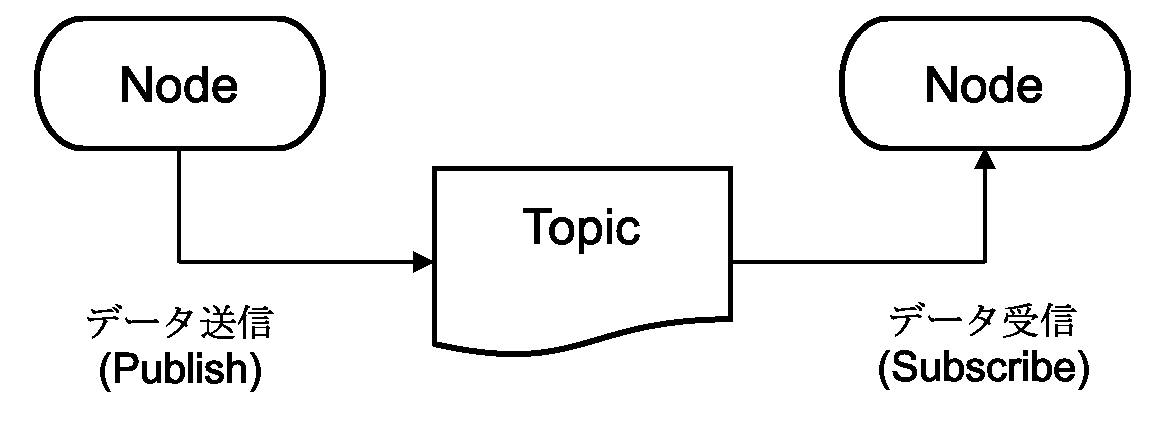
\includegraphics[width=0.5\hsize]{picture/eps/ros_topic.eps}
    \caption{ROSノードとトピックの概念}
    \label{fig::ros_topic}
\end{figure}



\begin{figure}[htb]
  \centering
    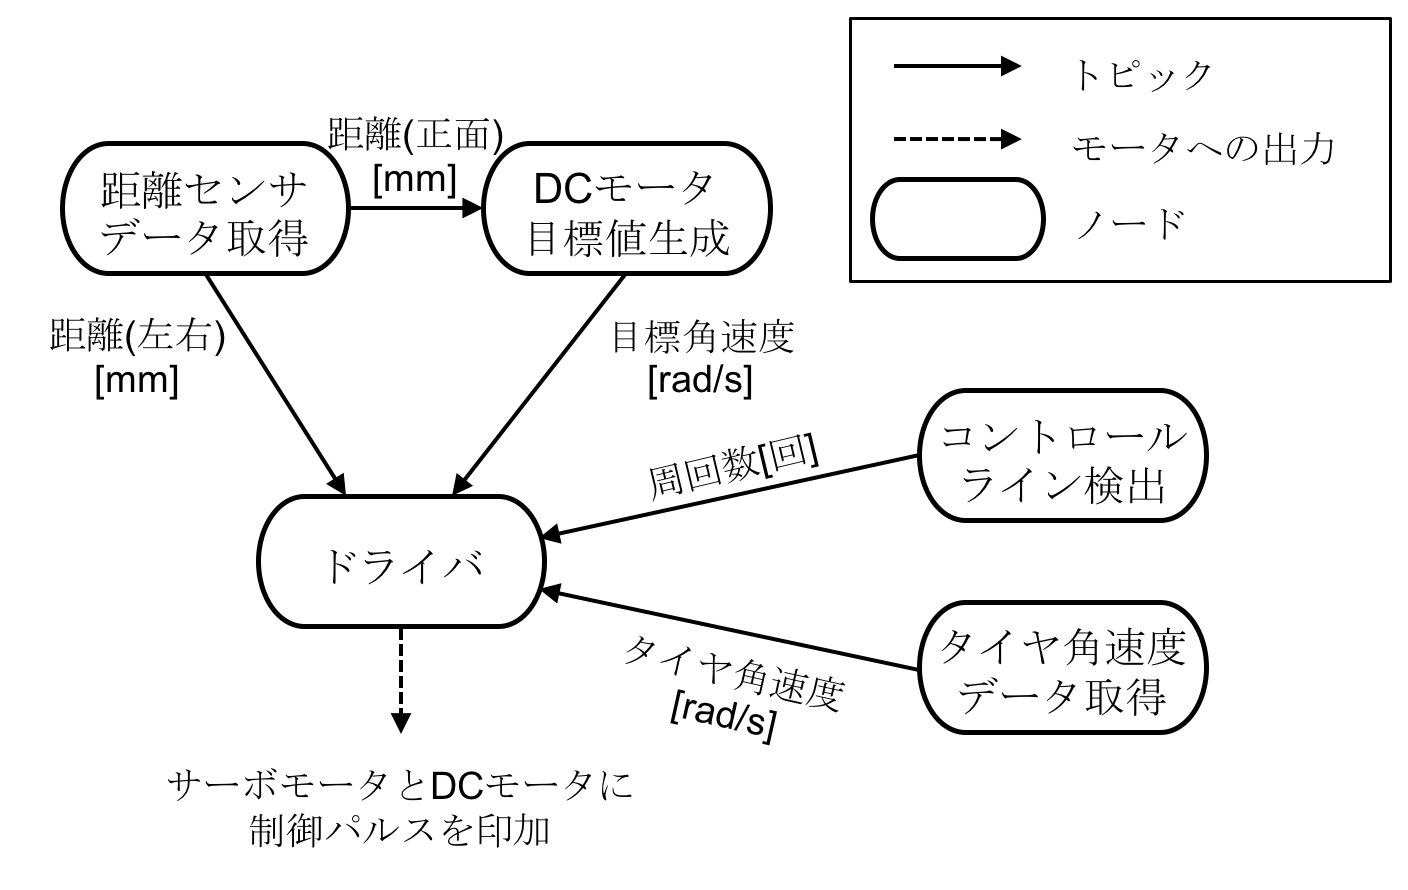
\includegraphics[width=0.8\hsize]{picture/eps/ros_nodes.eps}
    \caption{ROSノードとトピックの構成}
    \label{fig::ros_nodes}
\end{figure}

\newpage
\subsection{ROSノードとトピックの構成}
\refig{ros_nodes}に開発するROSノードとトピックの構成を示す.各ノードの役割は次の通りである.
\begin{description}

    \item[距離センサデータ取得] \mbox{} \\
      ロボカーの前方及び両側面に設置した距離センサからシリアルバス規格の一つである$\mathrm{I^2C}$を介して距離データを$\mathrm{[mm]}$単位で取得し外れ値処理や正規化を施した後にPublishする.
    \item[コントロールライン検出] \mbox{} \\
      ロボカーの後方下部に設置したフォトリフレクタによってコントロールラインを通過した回数をカウントしPublishする.

    \item[タイヤ角速度データ取得] \mbox{} \\
      ロボカーの後方に設置したロータリーエンコーダによって計測したタイヤの回転角を基に,タイヤの回転角速度を算出してPublishする.

    \item[DCモータ目標値生成] \mbox{} \\
      ロボカーの前方方向の距離データをSubscribeし,それをもとにDCモータに与える目標値を生成してPublishする.

    \item[ドライバ] \mbox{} \\
      DCモータに与える目標値,ロボカーの両側面の壁との距離,タイヤの角速度,周回数をSubscribeし,サーボモータの目標値を生成して,サーボモータを駆動させる.また,DCモータを目標値に追従するようなPI制御系によって駆動する.さらに,規定の周回数になるとロボカーを停止させる.


  \end{description}

\newpage
\section{制御則}
  ロボカーがコースを走る際,直進コースではロボカーを安定させ可能な限り速く走らせ,カーブに差し掛かったときにはステアリングとステアリングのための減速が必要である.特に,カーブを曲がりきるためにはどれだけのステアリング角と速度にすべきか,またその目標角度に追従させるためにはどのような制御系を構成する必要があるのかを考えなければならない.ここでは,ステアリング角と速度の目標値生成および制御方法について説明する.
 
 
\subsection{RCサーボモータ}
  ロボカーのステアリング角はRCサーボモータの角度により決められる.すなわち,RCサーボモータへの目標角度生成則について考える必要がある.
  
\subsubsection{構造}
RCサーボモータは内部でフィードバック制御が行われている.その構造は\refig{RC_construction}に示すとおりである\cite{RCservo}.目標角度に対応するPWM信号を入力すると内部で目標値に追従するように制御が行われる.

\subsubsection{目標値生成}
  本レースで走行させるロボカーは左右側面に設置された距離センサにより左右のコースの壁との距離をそれぞれ検出し,その距離の差によりステアリング角を変化させる.右側の壁との距離が左側の壁との距離より大きければステアリング角を時計回り方向に,小さければステアリング角を反時計回りに回転させる.ロボカーが直進コースを走行するときに比べ,カーブに差しかかったときとでは\refig{steering_compa}のように左右の壁との距離の差が大きくなる.すなわち,直進コースのように距離の差が小さくなるときにはRCサーボモータの角度を小さくしてロボカーが前方を向くようにし,大きくなるときにはRCサーボモータの角度を大きくすることでカーブに差しかかった場合に必要なステアリング角を実現することができる.また,直進コースではロボカーをコースの中央に位置させるようにステアリングを行わせることができる.
  
  RCサーボモータでのPWM信号の周期は$16〜23\unit{msec}$であり,その周期中のパルス幅の大きさに比例してRCサーボモータの角度が決まる.周期$20\unit{msec}$のPWM信号のパルス幅を$0.9\unit{msec}$から$2.1\unit{msec}$まで変化させると,RCサーボモータの角度は\refig{RC_pulse}に示すように変化する.この特性よりPWM信号のパルス幅$W\unit{msec}$に対してRCサーボモータの角度$\theta=f(W)\unit{\deg}$とおく.距離センサの値の定義域は正規化により$[0.0,1.0]$となるので,左右の距離センサの値の差は$[-1.0,1.0]$の範囲で値をとる.この範囲で左右の距離の差の大きさに応じてステアリング角を大きくし,最大角度を超えないようにする必要がある.そのためシグモイド関数$\sigma_{a_{s}}(x_{s}) $を用いた次式で目標角度$\theta_{r} $を生成することにした.

\begin{equation}  
  \theta_{r} = f(W) =f(1.5-2\cdot0.6(\sigma_{a_{s}}(x_{s})-0.5))
\end{equation}

\begin{figure}[htb]

  \centering
    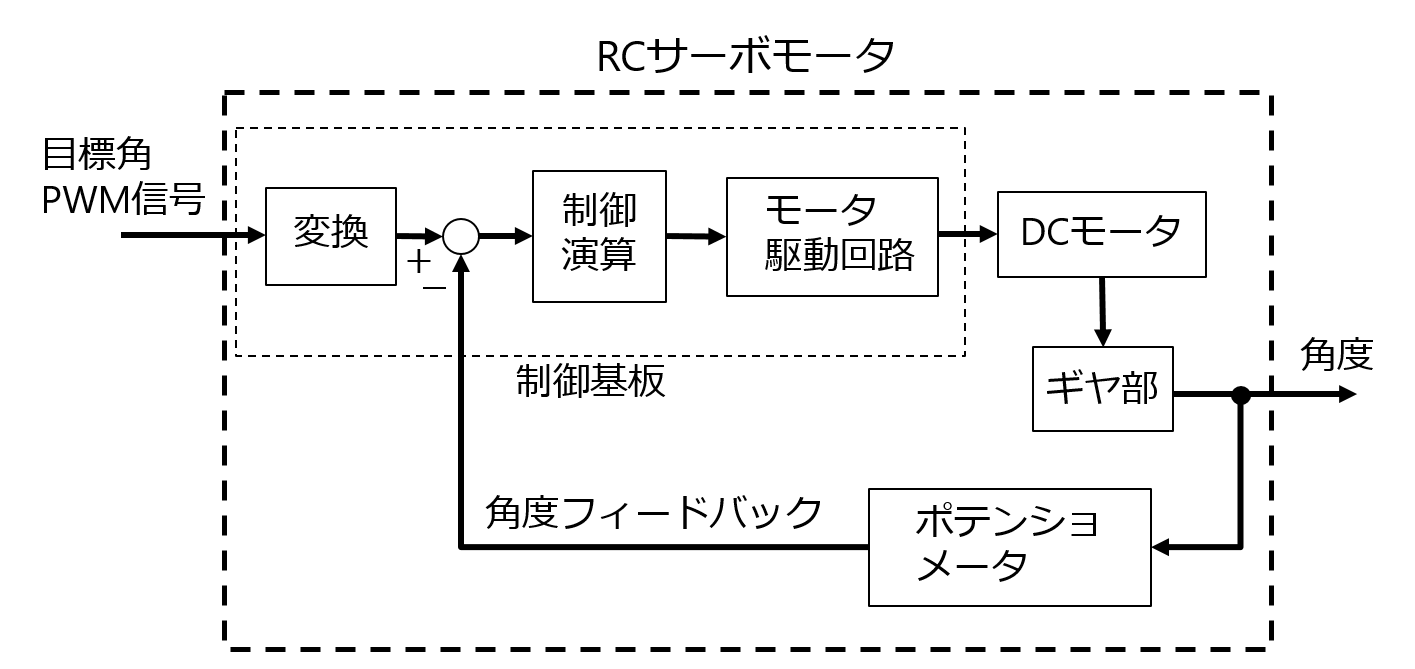
\includegraphics[width=0.7\hsize]{picture/eps/RC_construction.eps}
  \caption{RCサーボモータの制御系}
  \label{fig::RC_construction}
\end{figure} 

\begin{figure}[htb]

  \centering
    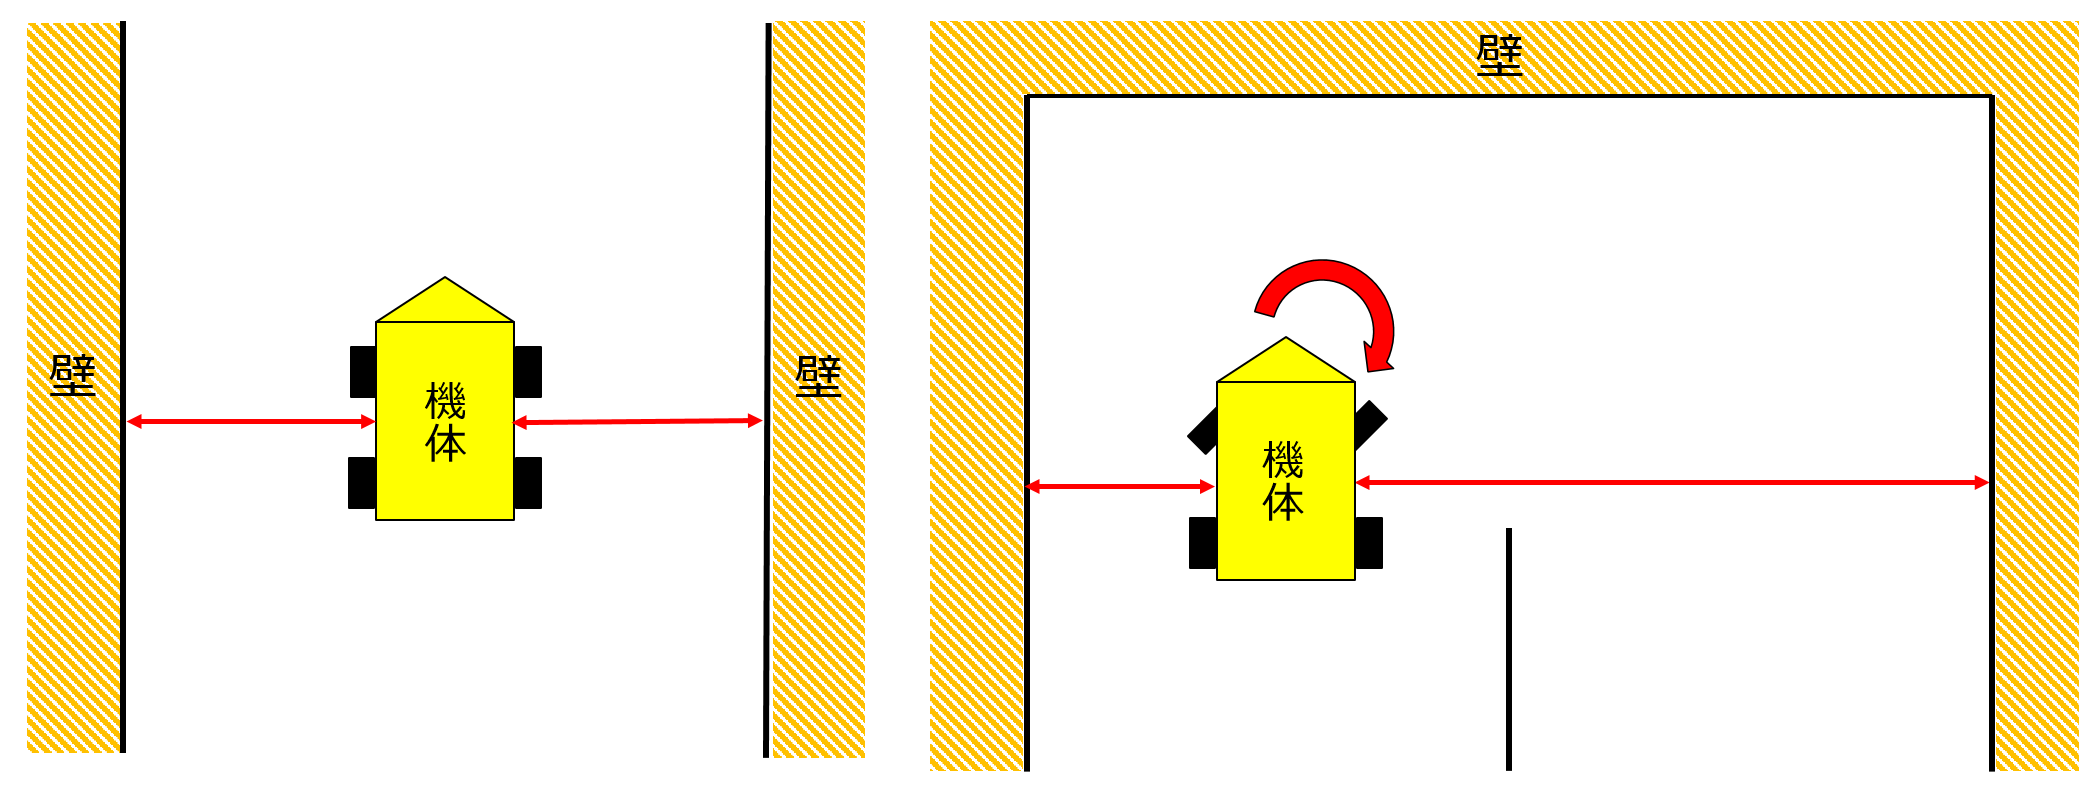
\includegraphics[width=0.8\hsize]{picture/eps/steering_compa.eps}
  \caption{直進コースとカーブとでの左右の壁との距離の差}
  \label{fig::steering_compa}
\end{figure}  

\begin{figure}[htb]

  \centering
    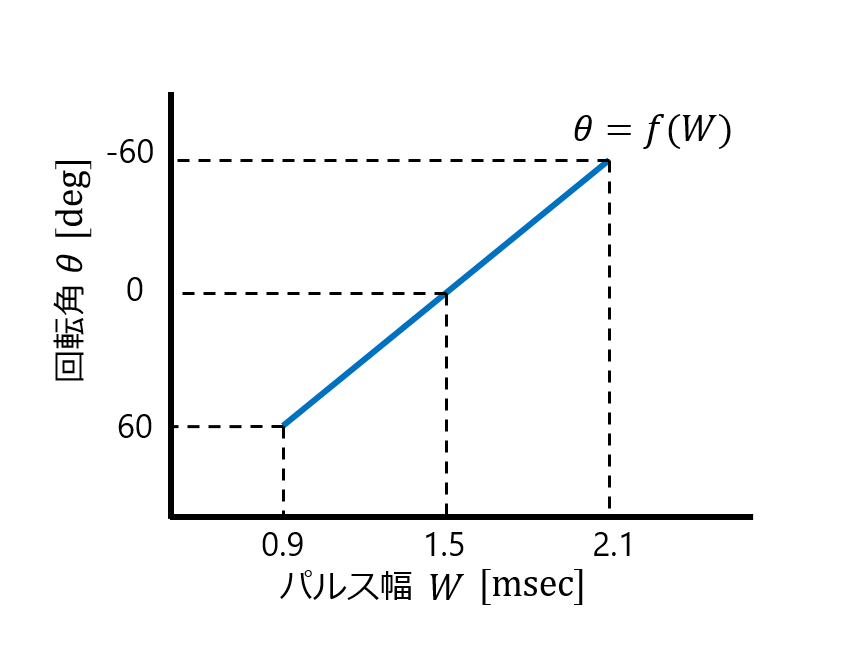
\includegraphics[width=0.5\hsize]{picture/eps/RC_pulse.eps}
  \caption{PWM信号のパルス幅とRCサーボモータの角度の関係}
  \label{fig::RC_pulse}
\end{figure} 
 
ここで$ a_{s}$は正の定数であり,$ x_{s}$はロボカーの左右のセンサの値の差である.この式ではシグモイド関数$\sigma_{a_{s}}(x_{s}) $を$y$軸方向に$-0.5$だけ平行移動させ,その全体を$2$倍することで$(-\infty,\infty)$の範囲において$(-1.0,1.0)$の値域で変化するようにしている.さらに,$0.6$をかけることで値域を$(-0.6,0.6)$としている.式中の$1.5$は\refig{RC_pulse}でRCサーボモータの角度が$0\unit{deg}$となるときのPWM信号のパルス幅である.この式では左右のセンサの値の差によりPWM信号のパルス幅を変えることで目標角度$\theta_{r} $を決定している.\refig{RC_pulse}に示したように,左右のセンサの値の差がなければ$x_{s}=0\unit{\deg}$となりパルス幅は$1.5\unit{msec}$となって目標角度$\theta_{r}$は$0\unit{\deg}$となる.右のセンサの値が左のセンサの値より大きい場合を正とすれば,RCサーボモータの角度は右の壁との距離の方が大きくなると時計回りに大きくなり,左の壁との距離のほうが大きくなると反時計回りに大きくなる.定数$a_{s}$はシグモイド関数の変化の速さにかかわり,試走実験を通して適切な値とする必要がある.

\subsection{DCモータ}
 ロボカーの速度はDCモータの角速度により決められる.すなわち,DCモータへの目標角速度生成と,その目標値に追従させるための制御方法を考える必要がある.

 \begin{figure}[htb]

  \centering
    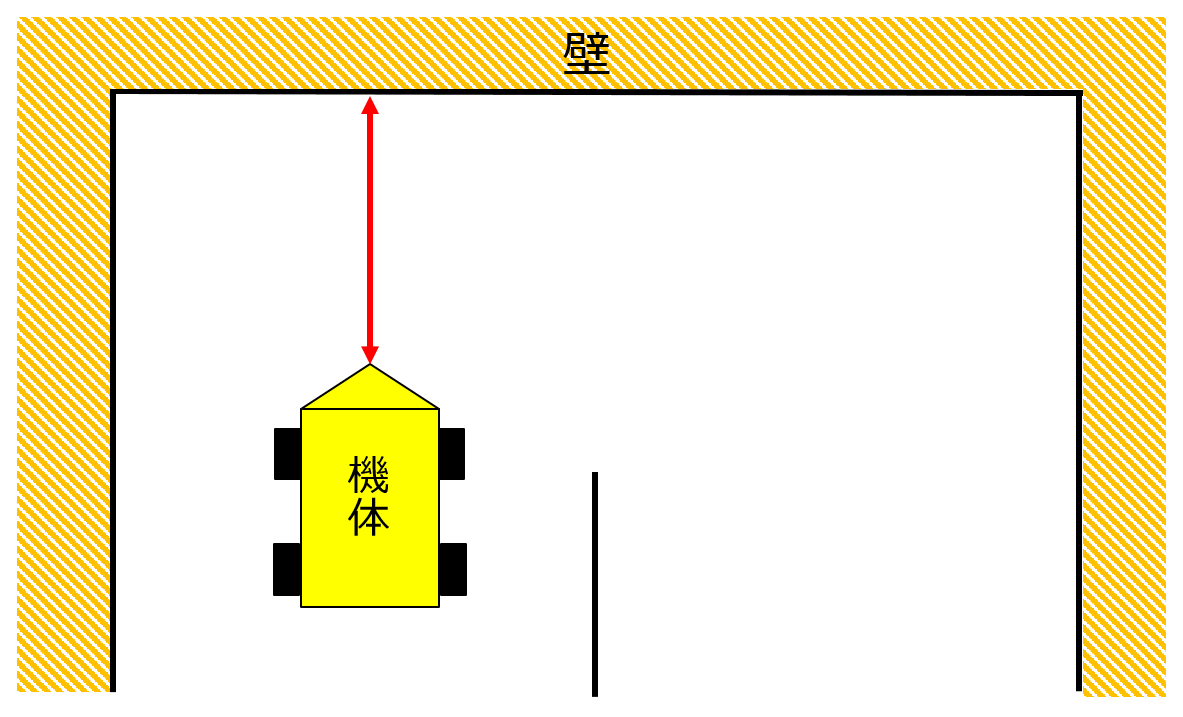
\includegraphics[width=0.6\hsize]{picture/eps/speed_wall.eps}
  \caption{前方の壁との距離に対する速度}
  \label{fig::speed_wall}
\end{figure}

\begin{figure}[htb]
  \centering
    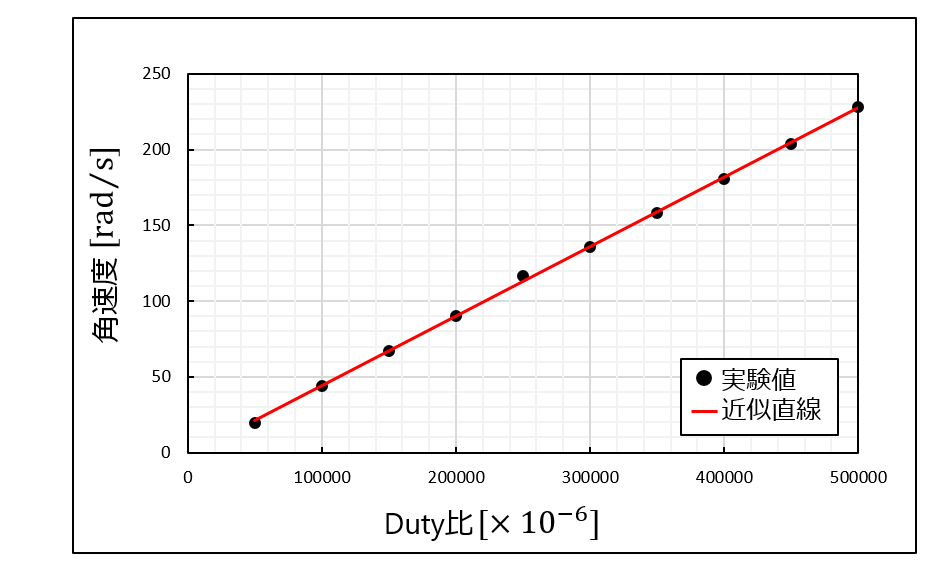
\includegraphics[width=0.7\hsize]{picture/eps/duty_angvel_graph.eps}
  \caption{PWM信号のDuty比とDCモータの角速度との関係}
  \label{fig::duty_angvel_graph}
\end{figure}

\subsubsection{PWM信号とDCモータの角速度}
 以下のようにして,PWM信号とDCモータの角速度との関係式を導いた.
\begin{enumerate}
\item DCモータにDuty比$0.05$のPWM信号を与え,定常となったときのDCモータの角速度の値を記録した.この値は定常時でのDCモータの角速度の値を平均化して求めた.なお,与えるDuty比はプログラムの関係上,実際のDuty比を$10^{6}$倍して与えている.
\item DCモータに与えるPWM信号のDuty比を$0.05$刻みで$0.5$まで増加させ,各Duty比の場合ごとに(1)と同様の操作を行った.
\item 各Duty比のPWM信号に対するDCモータの角速度は\refig{duty_angvel_graph}に示すようになった.これに対し近似直線を引けば,PWM信号のDuty比を$d[\times 10^{-6}]$,DCモータの角速度を$\omega\unit{rad/s}$とおいたときその式は
\begin{equation}
\omega=0.0005\times d-1.861 \label{eq::omega_pulse}
\end{equation}
と表せた.この式より,DCモータの角速度からPWM信号のDuty比を求める式は
\begin{equation}
d=2178\times\omega-4176 \label{eq::pulse_omega}
\end{equation}
と表せた.
\end{enumerate} 
\refeq{omega_pulse}よりPWM信号のDuty比が最大となったときのDCモータの角速度を求めることができ,\refeq{pulse_omega}より任意のDCモータの角速度を与えるのに必要なPWM信号のDuty比を求めることができる.
\subsubsection{目標値生成}
 カーブを曲がりきるためには,ステアリングに余裕をもたせる速度が必要である.本レースで走行させるロボカーは,正面に設置された距離センサにより前方の壁との距離を検出し,その距離に応じて速度を変化させる.\refig{speed_wall}のようにカーブに差しかかれば正面のコースの壁との距離は小さくなる.すなわち,正面のコースの壁との距離が小さくなるほどDCモータの角速度を小さくすることでカーブでの減速を実現することができる.壁との距離に比例して目標角速度を生成すると,壁との距離が大きくなるほどDCモータの角速度が大きくなりモータの最大角速度まで大きくなってしまう.DCモータの角速度が最大の状態でロボカーを走らせると消費電力が大きくなり電源の消耗が速くなったり,ロボカーがモータの回転に耐えられないなどの問題が生じる.この問題を解消するためには最大角速度をある値までに抑え,前方の壁との距離が一定以上大きくなるとそれ以上角速度が大きくならないようにする必要がある.なおかつ,壁との距離が小さくなれば速度を落としたいので,DCモータの角速度の目標値生成にはRCサーボモータと同様にシグモイド関数$\sigma_{a_{d}}(x_{d})$を用いることにした.指定最大角速度を$\omega_{max}\unit{rad/s} $とすれば,DCモータへの目標角速度$\omega_{r}\unit{rad/s}$は次式で生成される.
\begin{equation}
 \omega_{r}=\omega_{max}\sigma_{a_{d}}(x_{d}-b)\label{eq::omega_r}
\end{equation}
ここで,$a_{d}$,$b$は正の定数であり,$x_{d}$は前方の距離センサの値である.定数$a_{d}$はシグモイド関数の変化の速さに関わる.距離センサの値は正規化されているので$x_{d}$の定義域は$[0.0,1.0]$となる.シグモイド関数$\sigma_{a}(x)$は前方の壁との距離に対し増減し,値域は$(0.0,1.0)$である.センサの値が$0.0$のときにはシグモイド関数の値は$0.5$となる.これでは前方の壁との距離がどれだけ小さくなっても指定最大角速度の半分までしか減速できないため,指定最大角速度が大きくなるほど最低角速度が大きくなりステアリングのための減速が十分に行えなくなってしまう.正の定数$b$だけシグモイド関数を$x$軸方向に平行移動させることで,最低角速度を指定最大角速度の半分より小さくできる.以上より\refeq{omega_r}を与えることで,壁との距離がどれだけ離れても目標角速度$\omega_{r}\unit{rad/s}$は指定最大角速度$\omega_{max}\unit{rad/s}$に抑えられ電力消費を抑えることができ,前方の壁との距離が小さくなるカーブにおいてステアリングのための減速を行うことができる.正の定数$a_{d}$と$b$の値は試走実験を通して適切な値に決める必要がある.

\subsection{DCモータのモデリング}
DCモータの代表的な等価回路を\refig{dcm_circit}に示す.\cite{dcmmodeling}ただし,モータへの入力電圧を$v\unit{V}$,電機子電流を$i_{a}\unit{A}$,電機子抵抗を$R_{a}\unit{\Omega}$,自己インダクタンスを$L_{a}\unit{H}$,誘起電圧定数を$K_{E}\unit{Vs/rad}$,電機子の回転角速度を$\omega_{m}\unit{rad/s}$,電機子に発生するトルクを$T\unit{Nm}$,負荷トルクを$T_L\unit{Nm}$,回転子と負荷の合成慣性モーメントを$J\unit{kg\cdot m^2}$とする.以下ではこの等価回路に沿ってDCモータの定式化を行う.

\refig{dcm_circit}より,DCモータの支配方程式は次のように書ける.
\begin{align}
v &= K_{E}\omega_{m} + R_{a}i_{a} + L_{a}\frac{di_{a}}{dt} \label{eq::dcm_v} \\
T &= J\frac{d\omega_{m}}{dt} + T_{L} \label{eq::dcm_t}
\end{align}

\refeq{dcm_v},\refeq{dcm_t}より\refig{dcm_block}のブロック線図を得る.
ここで,図中の$J$はモータ回転子の慣性モーメント$J_{M}$と負荷の慣性モーメント$J_{L}$の和を表し,
$K_{T}\unit{Nm/A}$はDCモータのトルク定数である.
\refig{dcm_block}より負荷を含まないDCモータ単体の伝達関数$G_{M}(s)$を求めると以下のようになる.
\begin{align}
G_{M}(s) &= \frac{\Omega_{m}(s)}{V(s)} = 
\frac{\cfrac{K_{T}}{(R_{a} + L_{a}s)J_{M}s}}{1 + \cfrac{K_{T}K_{E}}{(R_{a} + L_{a}s)J_{M}s}} \nonumber \\
 &= \frac{\cfrac{1}{K_{E}}}{1 + \cfrac{R_{a}J_{M}}{K_{T}K_{E}}s + \cfrac{L_{a}J_{M}}{K_{T}K_{E}}s^2} \label{eq::dcm_tf}
\end{align}

ただし,$\Omega_{m}(s) = \mathcal{L}\{\omega_{m}(t)\},V(s) = \mathcal{L}\{v(t)\}$である.

\refeq{dcm_tf}より,電流の増加を遅らせるインダクタンスと回転角速度の上昇を遅らせる慣性モーメントという2つのエネルギ蓄積素子が二次のダイナミクスをつくっている事がわかる.

\begin{figure}[htb]
  \centering
    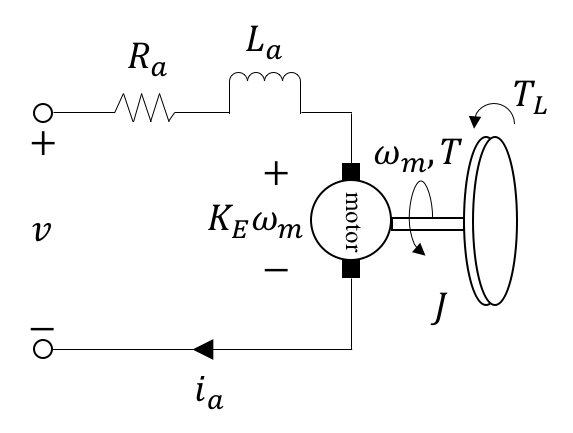
\includegraphics[width=0.5\hsize]{picture/eps/dcm_circit.eps}
    \caption{DCモータの等価回路}
    \label{fig::dcm_circit}
\end{figure}

\begin{figure}[htb]
  \centering
    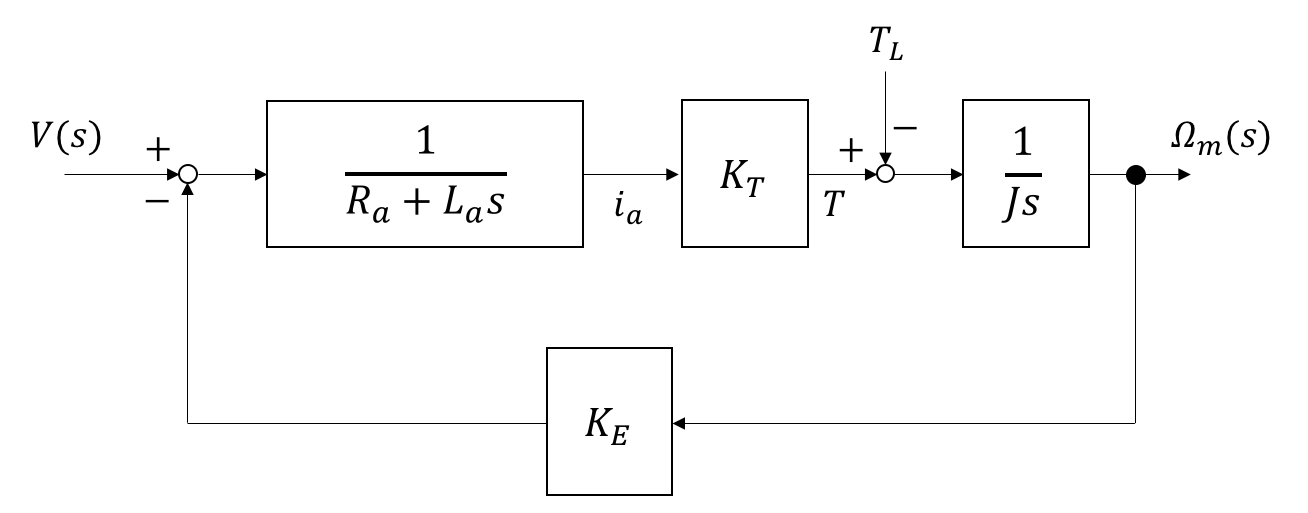
\includegraphics[width=1.0\hsize]{picture/eps/dcm_block_diagram.eps}
    \caption{DCモータのブロック線図}
    \label{fig::dcm_block}
\end{figure}
 

\subsubsection{制御系}
  DCモータの入力電圧から出力角速度への伝達関数を$G(s)$をとおく.DCモータの入力電圧から出力角速度への伝達関数は\refeq{dcm_tf}に示すように二次遅れ系となる.モデルを簡単にするためステップ応答法を用いて次式のように一次遅れ+むだ時間系に近似することにした.  
\begin{equation}
 G(s)=\frac{Ke^{-Ls}}{1+Ts}
\end{equation} 
$K$はゲイン,$T$は時定数,$L$はむだ時間である.ステップ応答法を用いて,以下のようにDCモータの入力電圧から出力角速度への伝達関数を求め,同定を行った.

\begin{enumerate}
\item 電圧$7.2\unit{V}$,Duty比$0.1$のPWM信号を加え,DCモータの角速度が定常になるまでの応答を記録した.この応答を\refig{dcmotor_response}に示す.このとき入力電圧は電圧とDuty比の積である$0.72\unit{V}$に相当し,定常での角速度は$30.74\unit{rad/s}$であるのでゲイン$K$は
\begin{equation}
 K=\frac{30.74}{0.72}=42.69
\end{equation}
となる.
\item (1)で得られた応答について,\refig{step_doutei}に示すように応答の変曲点で接線を引くことで時定数$T$とむだ時間$L$を求めた.$T$,$L$は以下の値となった.
\begin{align}
 T&=0.031 \\
 L&=0.006
\end{align}
\item(1),(2)よりDCモータの入力電圧から角速度への伝達関数は次式のようになった.
\begin{equation}
 G(s)=\frac{42.69e^{-0.006s}}{1+0.031s}
\end{equation} 
この伝達関数より同定した曲線を\refig{dcmotor_doutei}に示す.
\end{enumerate}

\begin{figure}[htb]
  \centering
    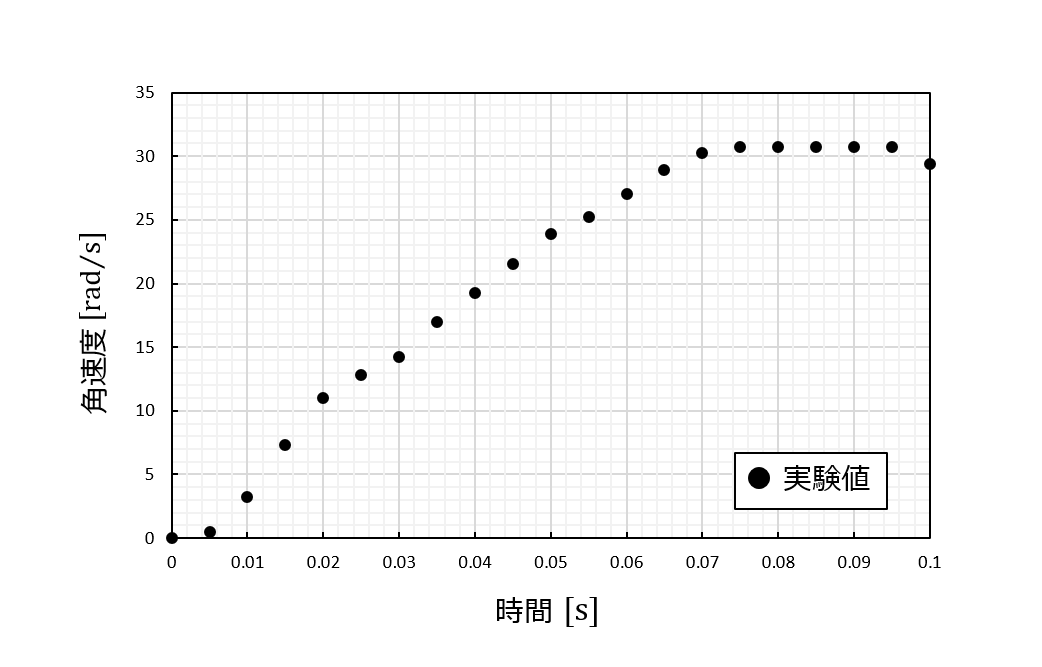
\includegraphics[width=0.7\hsize]{picture/eps/dcmotor_response.eps}
  \caption{DCモータのステップ応答}
  \label{fig::dcmotor_response}
  
\end{figure}

\begin{figure}[htb]
  \centering
    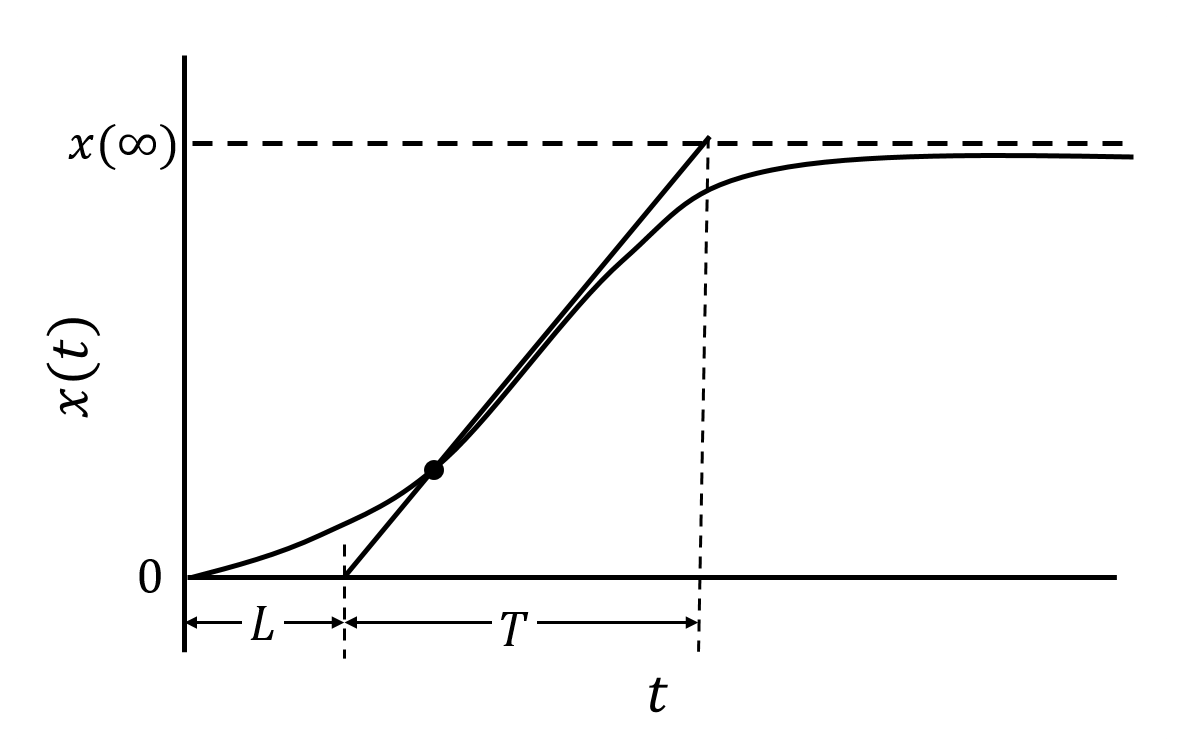
\includegraphics[width=0.7\hsize]{picture/eps/step_doutei.eps}
  \caption{ステップ応答から$T$と$L$を求める方法}
  \label{fig::step_doutei}
  
\end{figure}

\begin{figure}[htb]
  \centering
    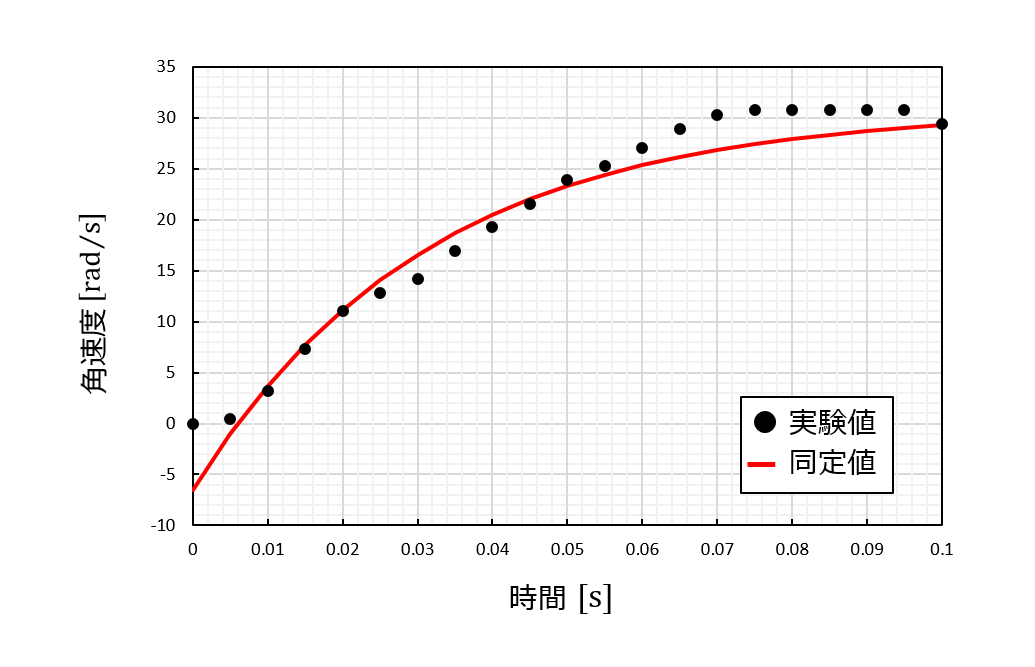
\includegraphics[width=0.7\hsize]{picture/eps/dcmotor_doutei.eps}
  \caption{DCモータの同定結果}
  \label{fig::dcmotor_doutei}
  
\end{figure}

  
  DCモータの制御系は,\refig{pi_control}に示すようにPI制御器を用いた閉ループ系で構成する.PI制御器を用いるのは,DCモータの角速度を目標角速度へ速やかに到達させるためである.PI制御器中の$K_{p}$,$K_{i}$は順に比例ゲイン,積分ゲインである.これらのパラメータの値をボード線図を用いて以下に決定した.
  まず,伝達関数$G(s)$とPI制御器のそれぞれについてボード線図での折れ点周波数を求めた.$G(s)$の折れ点周波数を$\omega_{1}$とおくと,その値は  
\begin{equation}
 \omega_{1}=\frac{1}{T}=32.25\unit{rad/s}
\end{equation}
となった.一方,PI制御器の折れ点周波数はPI制御器の式を
\begin{equation}
 K_{p}+\frac{K_{i}}{s}=K_{p}(1+\frac{\omega_{PI}}{s})
\end{equation}
と変形したときの$\omega_{PI}$である.ただし,
\begin{equation}
 \omega_{PI}=\frac{K_{i}}{K_{p}}\label{eq::omega_PI}
\end{equation}
である.

次に,伝達関数$G(s)$とPI制御器のそれぞれについてゲインと位相を求めた.
伝達関数$G(s)$,PI制御器のゲインをそれぞれ$g_{s},g_{PI}$,位相をそれぞれ$\phi_{s},\phi_{PI}$とおく.このとき$s=j\omega$とおけば,
\begin{align}
 g_{s}&=20\log_{10}{|G(j\omega)|}=20\log_{10}{\frac{K}{\sqrt{1+(\omega T)^{2}}}} \\
 \phi_{s}&=-\tan^{-1}{\omega T}-\omega L \\
 g_{PI}&=20\log_{10}{|K_{p}+\frac{K_{i}}{j\omega}|}=20\log_{10}{\sqrt{K_{p}^{2}+(\frac{K_{i}}{\omega})^{2}}} \\
 \phi_{PI}&=-\tan^{-1}{\frac{K_{i}}{K_{p}\omega}}
\end{align}
と各ゲイン,位相の式が求められた.ここで,PI制御器+伝達関数$G(s)$の開ループ伝達関数のゲイン,位相をそれぞれ$g_{c},\phi_{c}$とおく.これらの式は伝達関数$G(s)$とPI制御器のゲイン,位相をそれぞれ足し合わせて表せるので$g_{c},\phi_{c}$の式は
\begin{align}
 g_{c}&=g_{s}+g_{PI}\\
 \phi_{c}&=\phi_{s}+\phi_{PI}
\end{align}
となった.これらの式よりPI制御器+伝達関数$G(s)$のボード線図を描くことができる.

DCモータの角速度を目標値に追従させる制御を行うために以下のようにしてPI制御器+伝達関数$G(s)$のボード線図を描いた.

\begin{enumerate}
\item PI制御器+伝達関数$G(s)$のボード線図について,ゲイン交差周波数(ゲインが$0[dB]$となるときの角周波数)を$\omega_{c}$とおく.このとき,伝達関数$G(s)$の折れ点周波数$\omega_{1}$に対して,PI制御器の折れ点周波数$\omega_{PI}$は$\omega_{1}$より数倍程度小さく,$\omega_{c}$は数倍程度大きくなるように設定するようにした.一般にサーボ系ではゲイン余裕を$12~20\unit{dB}$,位相余裕を$40~60\unit{deg}$とするのがよいとされるので,これらの値を目安にして$\omega_{c}$,$\omega_{PI}$の値を変えることでゲイン余裕,位相余裕の値を調整した.また,$\omega_{c}$を大きくすれば速応性が大きくなるほど速くなるが,負荷の共振現象が存在する場合に負荷の振動を助長してしまうため大きくし過ぎないように設定することにした.これらの条件より
\begin{align}
 \omega_{PI}&=0.5\unit{rad/s}\label{eq::omega_PI_value}\\
 \omega_{c}&=120\unit{rad/s}\label{eq::omega_c_value}
\end{align}
とした.
\item ゲイン交差周波数$\omega_{c}$付近ではゲインの傾きが$-20\unit{dB/sec}$となるのが望ましく,角周波数がゲイン交差周波数$\omega_{c}$のときには次の等式が成り立つ.
\begin{equation}
|G(j\omega_{c})\cdot(K_{p}+\frac{K_{i}}{j\omega_{c}})|=1\label{eq::omega_c_1}
\end{equation}
\item \refeq{omega_PI_value},\refeq{omega_c_value}の値を用いて,\refeq{omega_PI},\refeq{omega_c_1}を連立して解くと,比例ゲイン$K_{p}$,積分ゲイン$K_{i}$は以下のように求まった.
\begin{align}
K_{p}&=0.090\label{eq::K_p_value}\\
K_{i}&=0.045\label{eq::K_i_value}
\end{align}
PI制御器のゲインをこのように設定したとき,PI制御器+伝達関数$G(s)$のボード線図は\refig{pi_board}に示すとおりである.このときのゲイン余裕,位相余裕は以下のとおりであった.
\begin{align}
ゲイン余裕:7.14\unit{dB}\\
位相余裕:63.6\unit{deg}
\end{align}
\refeq{K_p_value},\refeq{K_i_value}の値を用いたPI制御器では,一般にサーボ系で良いとされるゲイン余裕,位相余裕を得ることはできなかった.ゲイン交差周波数$\omega_{c}$付近でゲインの傾きを$-20\unit{dB/sec}$にでき,$\omega_{PI}$,$\omega_{c}$,$\omega_{1}$が互いに干渉しないようにボード線図を描けたのでこのPI制御器を用いて\refig{pi_control}のような閉ループ制御系を構成した.
\end{enumerate}
構成した閉ループ制御系に対して,DCモータの角速度追従実験を行った.目標角速度は$150\unit{rad/s}$とした.このときの応答を\refig{pi_response}に示す.応答は目標角速度$150\unit{rad/s}$に$0.3\unit{s}$で到達して定常となった.これより,目標角速度への追従が実現できたといえる.

\begin{figure}[htb]
  \centering
    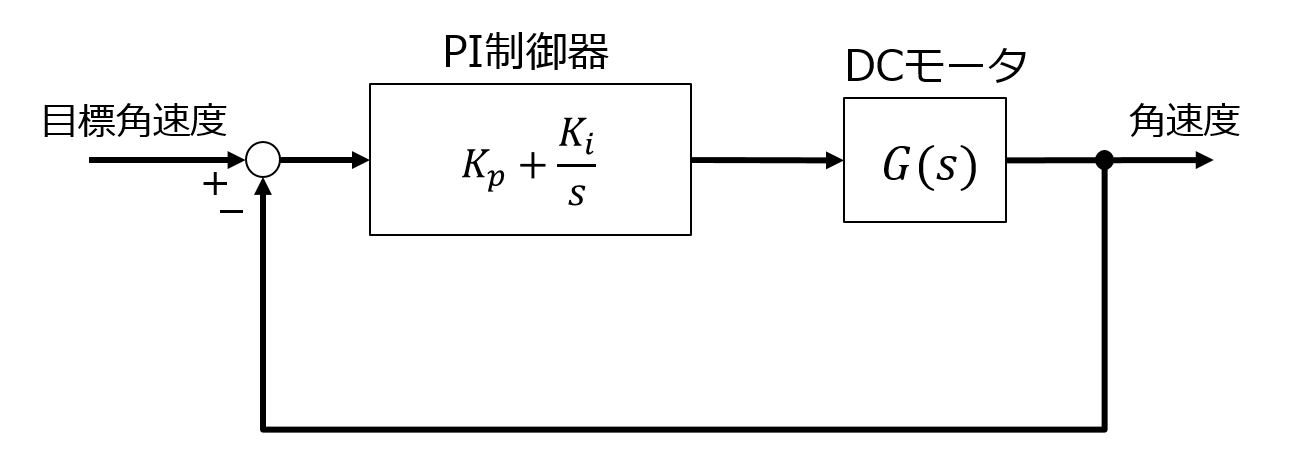
\includegraphics[width=0.7\hsize]{picture/eps/pi_control.eps}
  \caption{DCモータの制御系}
  \label{fig::pi_control}
  
\end{figure}

\begin{figure}[htb]
  \centering
    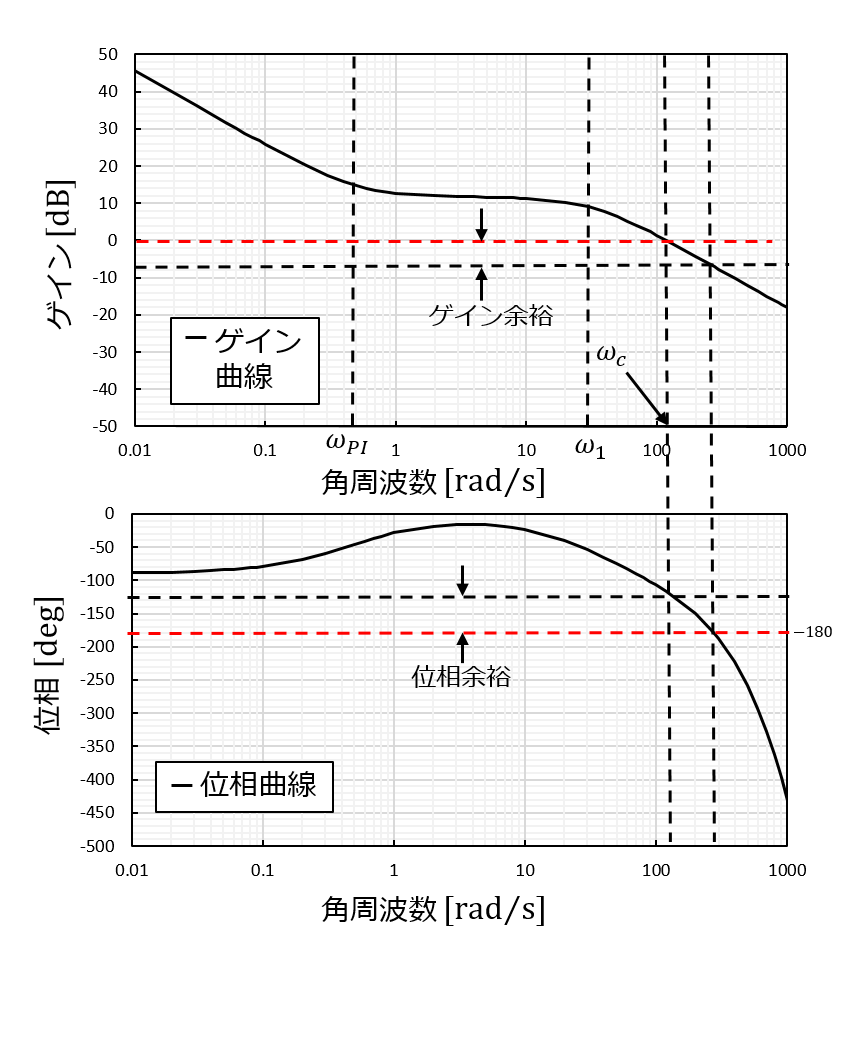
\includegraphics[width=0.7\hsize]{picture/eps/pi_board.eps}
  \caption{PI制御器+伝達関数$G(s)$のボード線図}
  \label{fig::pi_board}
  
\end{figure}

\begin{figure}[htb]
  \centering
    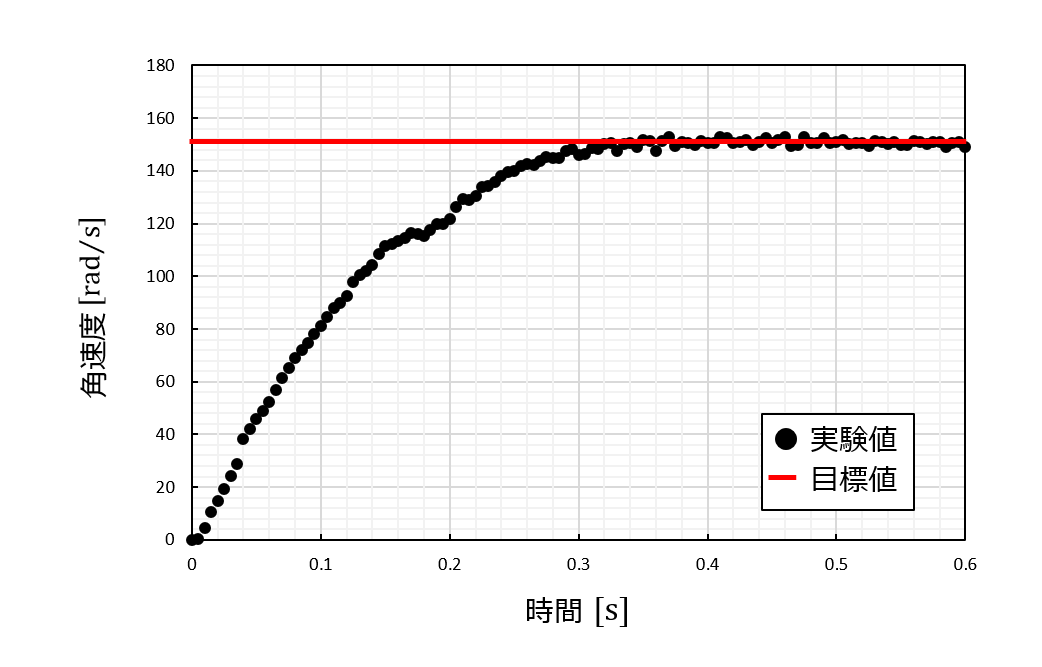
\includegraphics[width=0.7\hsize]{picture/eps/pi_response.eps}
  \caption{閉ループ制御系の応答}
  \label{fig::pi_response}
  
\end{figure}

\newpage
\section{結果}
以下に,走行会における走行結果を示す.走行成功時の最速タイムは48.5秒であった.
\begin{description}

    \item[1回目] \mbox{} \\
      走行失敗.2週目の終盤のカーブでセンサ異常により壁に衝突した.
      
    \item[2回目] \mbox{} \\
      走行成功.

    \item[3回目] \mbox{} \\
      走行成功.ただし,走行開始直後でコントロールラインの検出に失敗したため,3周回った後に停止.また,2回目の走行時よりもタイヤの目標角速度を高く設定したところ,コース周回中に一時的にステアリング制御が不安定になり,振動を起こしている場面があった.


  \end{description}
\section{考察}
ここでは1回目の走行において壁に衝突した原因,3回目の走行においてコントロールラインを一回検出し損ねた原因,またステアリング制御が振動を起こした原因の3点について考察していく.

\subsection{壁に衝突した原因}
1回目の走行では,2周目の終盤までは安定して走行していたが,終盤のU字カーブでステアリングを切ることなく壁に衝突した.この時,一切ステアリング動作をしていなかったため,距離センサの異常により距離データの取得に失敗していたと考えられる.距離センサの異常原因としてRaspberryPi3 Model BのCPU負荷が大きくなりすぎてしまったことや,振動等により配線の接触不良が発生したこと等が考えられる.

\subsection{コントロールラインを検出し損ねた原因}
我々のロボカーは,フォトリフレクタを用いてコントロールラインを検出する際に,ロバスト性向上のためにフォトリフレクタから100回データを取得し,その平均がしきい値を超えたかどうかでコントロールラインの白色部をを通過したかどうかを検出していた.そのため,コントロールラインを通過する速度,位置,タイミングによっては,100回計測している間に白色部を通過してしまい,コントロールラインの検出が正しく行えなかった可能性があると考えられる.

\subsection{ステアリング制御が振動を起こした原因}
我々が使用した距離センサはセンサの仕様上,距離の測定に最速でも$20\unit{ms}$かかる.今回,ロボカーにはこの距離センサを3つ搭載し,それぞれのセンサで距離を測定した後にその距離データに応じて機体を制御していた.すなわち,制御周期は最速でも$60\unit{ms}$はかかることになる.さらに,実際には他の処理による遅延も含まれるため,より制御周期は遅くなっていたと考えられる.これにより,タイヤの目標角速度を高く設定した時に制御周期が追いつかなくなってしまい,振動を起こしてしまったと考えられる.
\section{感想と次年度への提言}
今回,私は主にロボカーのソフトウェア開発とチーム全体の統括を担当した.そこで最も痛感した点はプロジェクトマネジメントの大変さである.RCRはチームで進めるプロジェクトであり,円滑なプロジェクト進行には,各メンバ間での進捗状況や意見等の共有が不可欠である.しかし今回は,あるメンバの仕事が終わらないと他のメンバの仕事に着手できないという状況を生んでしまったり,一部のメンバに仕事が集中してしまい,他のメンバにその進捗状況がうまく伝わらなかった等といった様々な問題が生じてしまった.

主な原因として,例年に比べ10人と人数が多くチームが大きくなりすぎた点,時系列を意識した役割ないし仕事の分担が出来ていなかった点,大学院一般入試の有無や経験の差などによって全メンバに平等に仕事を割り振ることが難しくなった点,そしてミーティングでその差を十分に埋めきれず,各メンバ間で理解度に差が生じてしまった点等が挙げられる.

また今年度は,機体のベースが配布されたことにより例年よりも発表内容が少なくなったことに加え,人数が多かったため,発表の際に一人あたりの分量が少なくなってしまい,かつ内容が細かく分割されるため,聴衆に伝わりやすいスライド構成にすることが難しかった.プレゼンテーションの評価のために全員発表にしなければならないと言った事情はもちろん承知しているが,来年以降はこの点に多少なりとも何かしらの配慮があれば良いと考える.
\newpage
\section{物品一覧}
今回の配布品,引継ぎ品,購入品についてそれぞれ,以降の表にまとめる.
\begin{table}[h]
	\centering
	\caption{配布品一覧}
	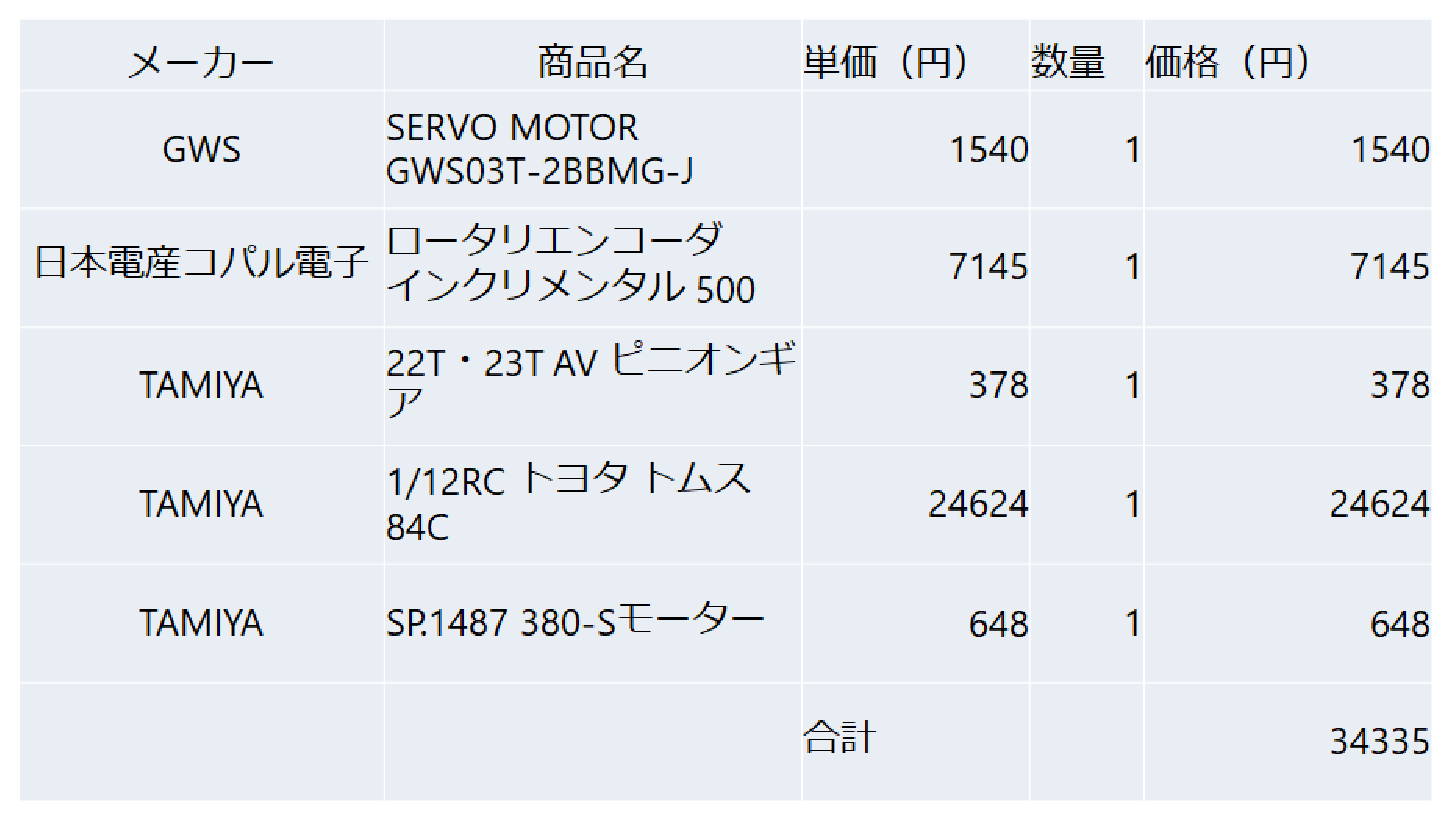
\includegraphics[clip,scale=0.4]{picture/eps/distributed_part.eps}
    \label{distribution}
\end{table}

\begin{table}[h]
	\centering
	\caption{引継ぎ品一覧}
	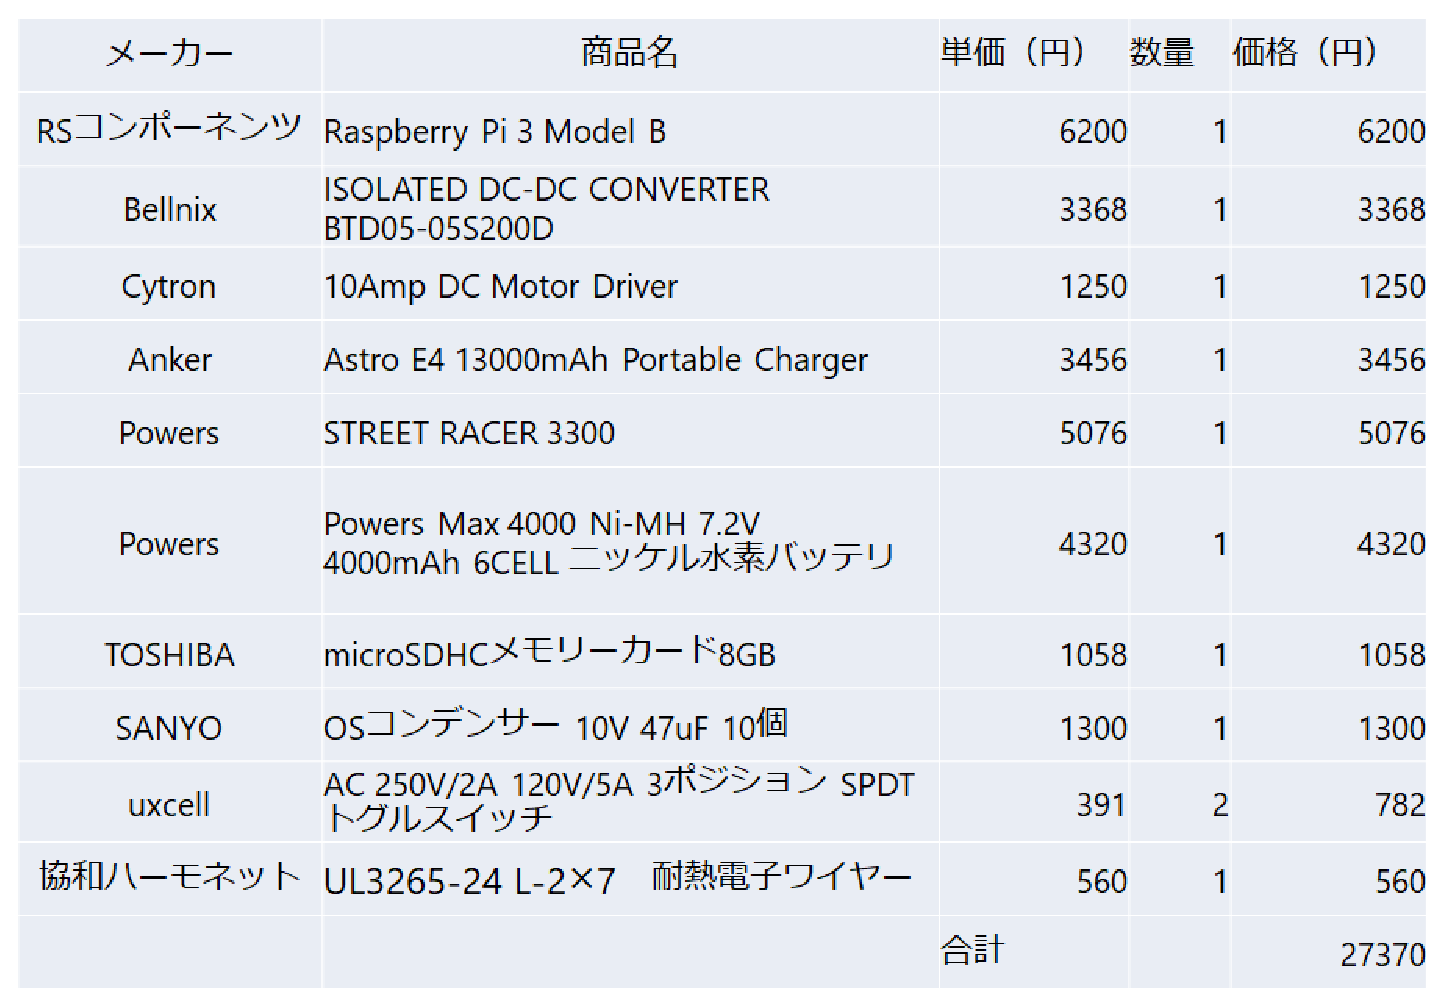
\includegraphics[clip,scale=0.4]{picture/eps/old_part.eps}
 \label{old}
\end{table}

\begin{table}[h]
	\centering
	\caption{購入品一覧}
	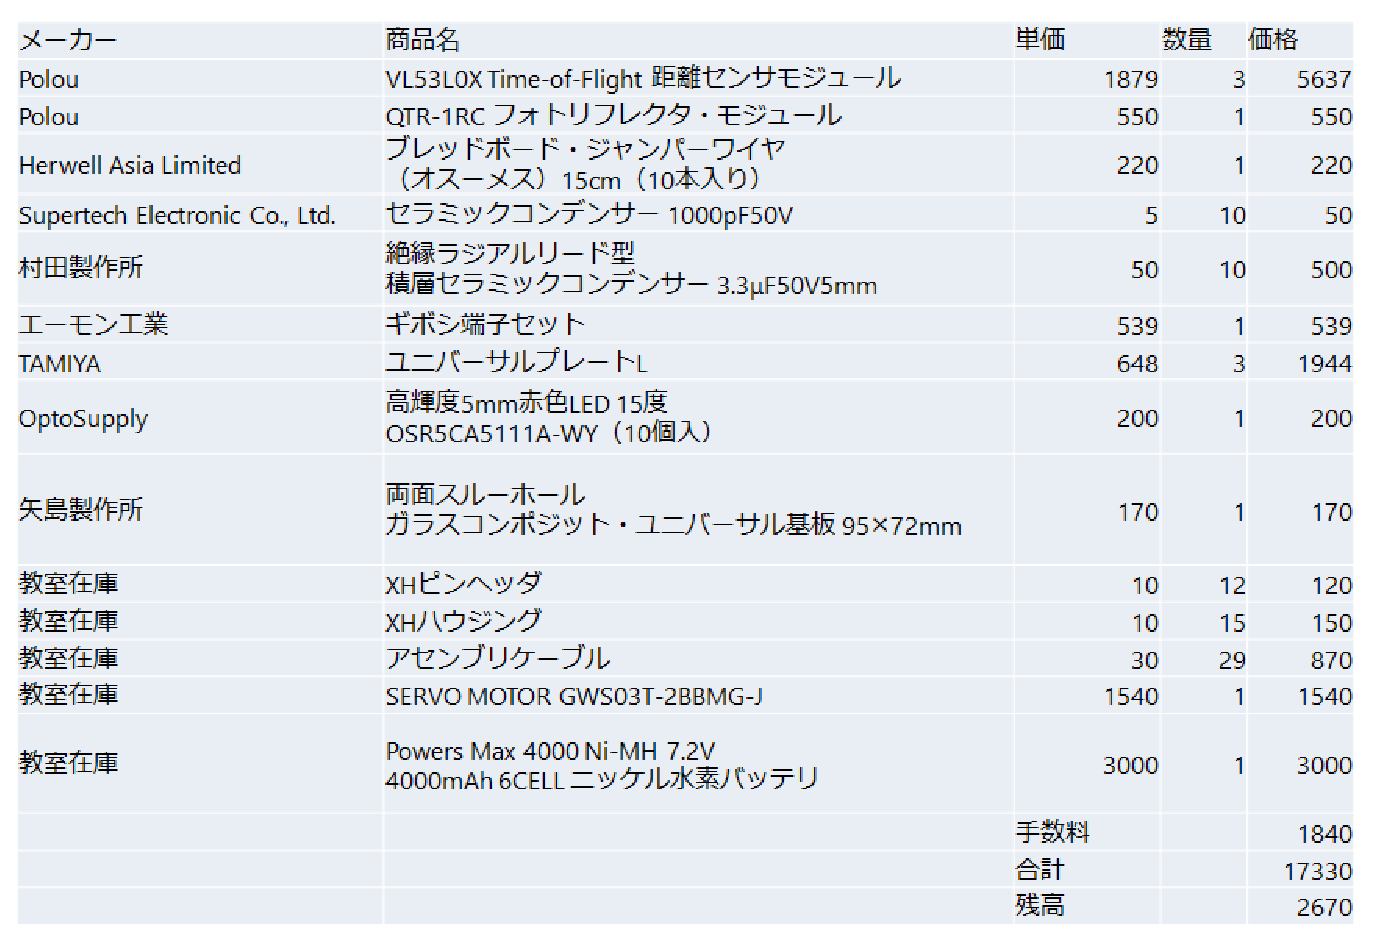
\includegraphics[clip,scale=0.4]{picture/eps/new_part.eps}
    \label{new}
\end{table}

\newpage

\begin{thebibliography}{99}
  \bibitem{tof_sensor1}
  SWITCH SCIENCE, "Pololu VL53L0X Time-of-Flight 距離センサモジュール"
  \textless https://www.switch-science.com/catalog/2869 \textgreater
  2018年6月1日アクセス.
  
  \bibitem{i2c}
  Philips\quad Semiconductors,\quad "$\mathrm{I^2C}$\hspace{0.5em}バス仕様書バージョン2.1"          
  \textless http://ekousaku.web.fc2.com/doc/I2C.pdf \textgreater
  \quad 2018年6月1日アクセス.

 \bibitem{kurazume}
    表允晳,倉爪亮,渡邊裕太, "詳説 ROSロボットプログラミング-導入からSLAM・Gazebo・MoveItまで-", 
    Kurazume Laboratory, pp.15-18, (2015).

  \bibitem{ogura}
    小倉崇, "ROSではじめるロボットプログラミング", 工学社, pp.8-10, (2015).
  
  \bibitem{motor} 
  後閑哲也, "作る,できる/基礎入門 電子工作の素", 技術評論社, p181, (2009).
  
  \bibitem{motordriver} 
  Cytron technologies, "MD10C Enhanced 10Amp DC Motor Driver User's Manual Rev2.0 v1.0", 
  \textless https://www.robotshop.com/media/files/PDF/user-manual-md10c-v2.pdf\textgreater , 2018年6月2日アクセス.
  
  \bibitem{R380} 
  MABUCHI MOTOR, "Let's Motorize",\\
  \textless https://www.mabuchi-motor.co.jp/motorize/branch/motor/ \textgreater , 2018年6月3日アクセス.
  
  \bibitem{dcdcconverter} 
  SWITCH SCIENCE, "10Watt BTD Series", 
  \textless http://www.bellnix.co.jp/pdf/pdf/BTD.pdf\textgreater , 2018年6月2日アクセス.
  
  \bibitem{dcdc} 
  後閑哲也, "作る,できる/基礎入門 電子工作の素", 技術評論社, pp.84-85, p186, (2009).
  
  \bibitem{pololu}
   Pololu\quad Corporation,\quad "QTR-1RC\quad Reflectance\quad Sensor(2-Pack)",
   \textless https://www.pololu.com/product/2459 \textgreater , 2018年6月1日アクセス.
  
  \bibitem{RCservo}
  Interface,"実験研究!サーボモータの応答特性",\\
  \textless http://www.kumikomi.net/interface/sample/201407/if07\_ 108.pdf\textgreater ,\\
  2018年6月25日アクセス.  
  
  \bibitem{dcmmodeling}
    坂本哲三, "電気機器の電気力学と制御", 森北出版, pp.164-168, (2007).
  

\end{thebibliography}

\end{document}
